\section{CSR-Based Formats and Algorithms for \spmv}
\label{sec:spmv}


CSR represents a sparse matrix $A \in \R^{m \times n}$ in compact form
using three arrays:
vector {\tt val} stores the $n_z$ non-zero values by rows;
{\tt colidx} keeps the column index for each value in the same order;
and {\tt rowptr} contains $m+1$ row pointers that mark the initial
and final position of each row within the other two arrays;
see Figure~\ref{2017-csr-spmv:fig:spmv}.
Storing the sparse matrix $A$ in CSR format thus requires ${\cal S}_{CSR} = n_z(s_v+s_i)+(m+1)s_i$ bytes, where
$s_v$ and $s_i$ respectively denote the number of bytes occupied 
by each value and integer index.

\begin{figure}[t]
\begin{tabular}{c}
\begin{minipage}{\textwidth}
\begin{center}
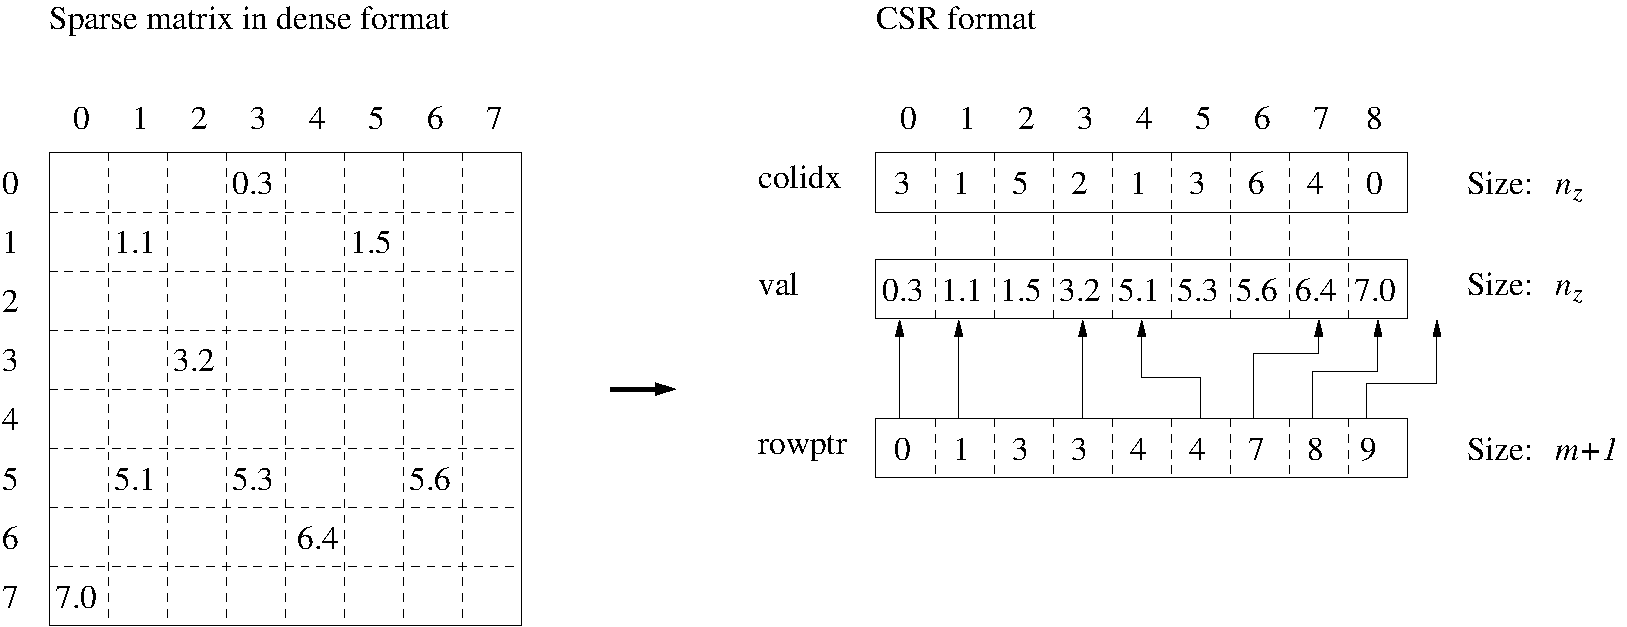
\includegraphics[width=\textwidth]{plots/csr_format}
\end{center}
\end{minipage}
\end{tabular}
\caption{Data layouts
for an $8 \times 8$ sparse matrix with $n_z$=9 nonzero entries.}
\label{2017-csr-spmv:fig:spmv}
\end{figure}

In~\cite{Bell:SpMV:NVIDIA:2008}, Bell and Garland (BG) explored the performance
of different sparse formats and implementations of \spmv for throughput-oriented GPUs from NVIDIA.
BG's \spmv kernels based on CSR
parallelize the product
across the matrix rows,
with one CUDA thread assigned to each row in the {\em scalar} kernel (CSR-s) or,
alternatively, one warp per row in the {\em vector} kernel (CSR-v).
CSR-s has two major issues though: first, for sparse matrices with an
irregular row distribution of their non-zero entries,
many threads within a warp will likely remain idle.
Second, since each thread of a warp works on a different row,
the memory accesses are noncoalesced.
CSR-v aims to amend the second issue,
though it
requires that the rows contain a number of nonzeros greater than the warp
size in order to deliver high performance~\cite{Bell:SpMV:NVIDIA:2008}.

A couple of examples illustrate the advantages/deficiencies
of CSR-s and CSR-v.
Consider first an arrowhead matrix,
with all its nonzero entries lying on the main diagonal
and the last column/row of the matrix.
(This problem type appears in domain decomposition methods,
when discretizing partial differential equations.)
This matrix structure poses an ill-case scenario for both BG kernels,
as it produces a highly unbalanced mapping of the workload to the threads.
In contrast, a tridiagonal matrix
(often encountered in computational physics),
results in an almost perfectly balanced distribution
of the workload for both BG CSR kernels,
but yields a significant waste of resources for CSR-v.

Figure~\ref{fig:motivation} provides a motivating example for our work.
The left-hand side plot there shows the sparsity pattern for matrix
{\sc Freescale/transient} from the SuiteSparse Matrix Collection.%
\footnote{Formerly known as the University of Florida Matrix Collection:
\mbox{\url{http://www.cise.ufl.edu/research/sparse/matrices/}}.}
The distribution of the nonzeros for this problem,
arising in circuit simulation, shows quite an unbalanced pattern,
with most of the elements concentrated in a few rows of the matrix.
Concretely, more than 95\% of the rows contain 10 or less nonzeros;
99.95\% comprise 100 or less nonzeros;
only 5 rows contain more than $10^3$ nonzeros; and only 2 more than $10^4$,
with the densest row comprising
60,423 nonzero entries.

The right-hand side plot in Figure~\ref{fig:motivation}
reports the execution time on an NVIDIA GTX1080 GPU
for double-precision \spmv kernels based on CSR and HYB
(implemented in cuSPARSE~\cite{cusparse}),
SELL-P (from MAGMA-sparse\footnote{
\mbox{\url{http://icl.cs.utk.edu/magma/}}.}),
and our balanced version of CSR (\bcsr).
ELL and ELLR-T are not included because,
for this problem instance, they both need to store an
$m \times 60,423$ matrix just for the array {\tt val}
(i.e., more than 79.5~Gbytes in double precision),
which exceeds the memory of the target GPU.
For this particular matrix both CSR and SELL-P exhibit poor performance
compared with HYB and CSR-I. SELL-P also suffers
from considerably higher memory consumption than other implementations.
CSR-I is the best performing algorithm in this case,
achieving slightly better performance than HYB,
while maintaining the storage efficiency of CSR.

\begin{figure}[t]
\begin{center}
\begin{tabular}{cc}
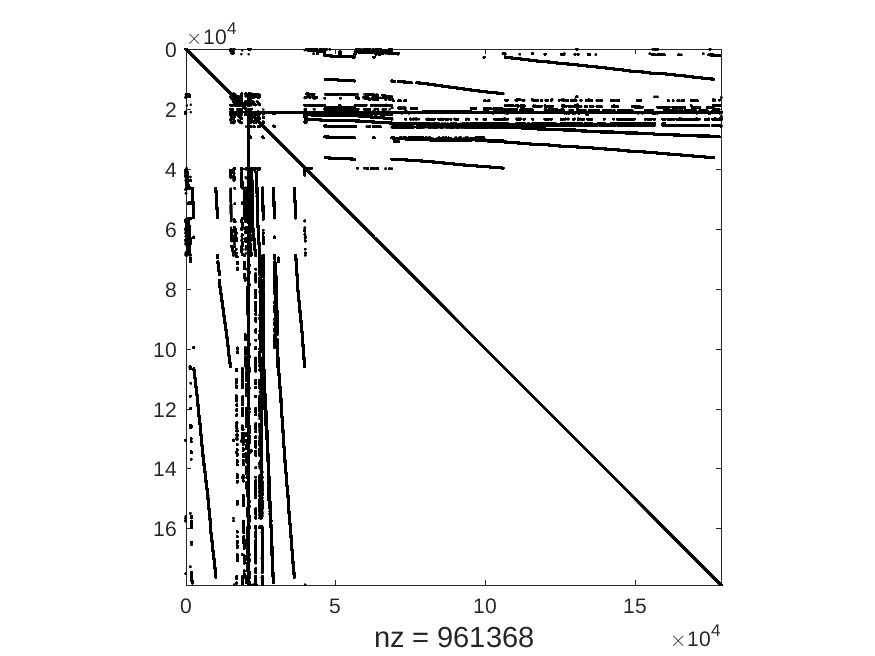
\includegraphics[width=0.48\textwidth]{plots/pattern.pdf} &
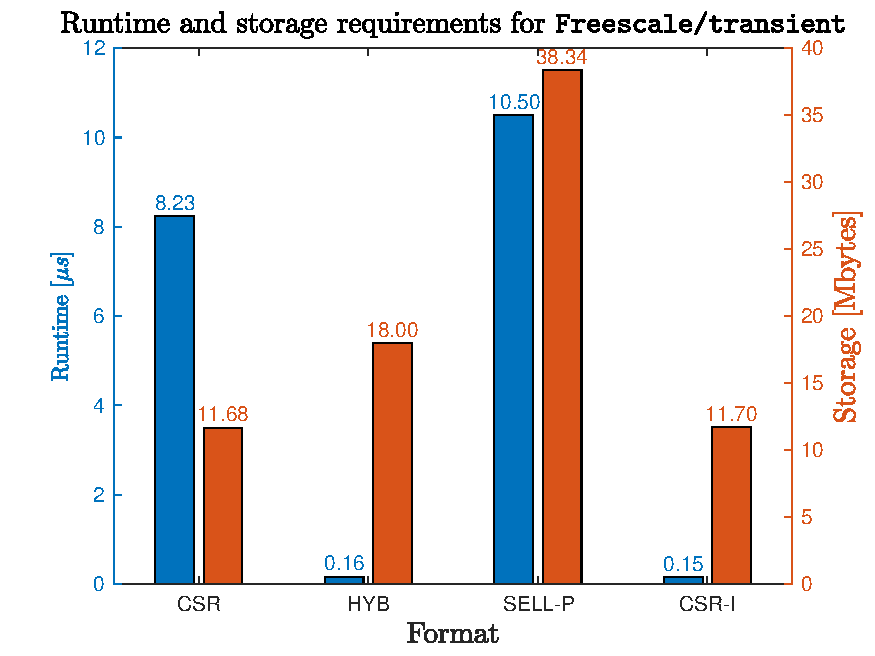
\includegraphics[width=0.48\textwidth]{plots/motivation.pdf}
\end{tabular}
\end{center}
\vspace*{-2ex}
    \caption{Left: sparsity pattern for {\sc Freescale/transient}.
    Right: execution time (blue) and memory consumption (red) on a GTX1080
    using different \spmv kernels.}
\label{fig:motivation}
\end{figure}

